\documentclass[leqno]{article}
\usepackage[left=0.5in,right=0.5in]{geometry}
\usepackage[utf8]{inputenc}
\usepackage{amsmath, amsfonts, color, booktabs, centernot, graphicx, fancyhdr}
\setlength\parindent{0pt}
\begin{document}
\title{Noisy Observations Simulation}
\author{Leah Dickstein}

\maketitle
\section*{Setup}
\begin{align*}
\textbf{System} \quad x(n) &= ax(n-1)+w(n-1)\\
y(n) &= cx(n)+v(n)\\
&\\
x(0) &\sim N(0,1)\\
w(n-1) &\sim N(0,\sigma_w^2)\\
v(n) &\sim N(0,\sigma_v^2)\\
&\\
\textbf{Distribution}: &\quad \frac{N(cx[n],\sigma_v^2)N(0,a^{2n}+\sigma_w^2\sum_{i=0}^{n-1}a^{2i})}{N(0,c^2a^{2n}+c^2\sigma_w^2\sum_{i=0}^{n-1}a^{2i}+\sigma_v^2)}\\
&\\
\hat{x}[n] &= \frac{yc(a^{2n}+\sigma_w^2\sum_{i=0}^{n-1}a^{2i})}{c^2(a^{2n}+\sigma_w^2\sum_{i=0}^{n-1}a^{2i})+\sigma_v^2} = \frac{yc\sigma_x^2}{\sigma_y^2}
\end{align*}

\section*{Code (MatLab)}
\begin{verbatim}
clc;
clear all;
set(0,'DefaultAxesFontSize', 14);

a = 1; %Test 2,0.5,10
c = 1;
varv = 1;
varw = 1;

%initialize
x = normrnd(0,1,[1,1]); %x[0]
y = c*x+normrnd(0,varv);
xhat = y*c*1/(c^2+varv);
varx = 1;

%time passing
for n=1:10
    w = normrnd(0,varw);
    x = [x a*x(1,n)+w];
    v = normrnd(0,varv);
    y = [y c*x(1,(n+1))+v];
    varx = a^2*varx + varw;
    vary = c^2*varx + varv;
    xhat = [xhat y(1,n+1)*c*varx/vary];
end

%hold all
subplot(1,2,1), stem(0:10,x,'k','filled')
subplot(1,2,1), hold on, stem(0:10,y,'b')
subplot(1,2,1), hold on, stem(0:10,xhat,'r')
xlabel('n=time')
legend1 = legend('x','y','xhat','Location','Best');

subplot(1,2,2), stem(0:10,y/c-x,'b')
subplot(1,2,2), hold on, stem(0:10,xhat-x,'r','filled')
xlabel('n=time')
legend2 = legend('y/c-x','xhat-x');

suptitle(['a= ' num2str(a) '; c= ' num2str(c) '; varv= ' num2str(varv) '; varw= ' num2str(varw)])
\end{verbatim}

\pagebreak
The initial setup is a=1, c=1, varw = 1, varv = 1.
\begin{center}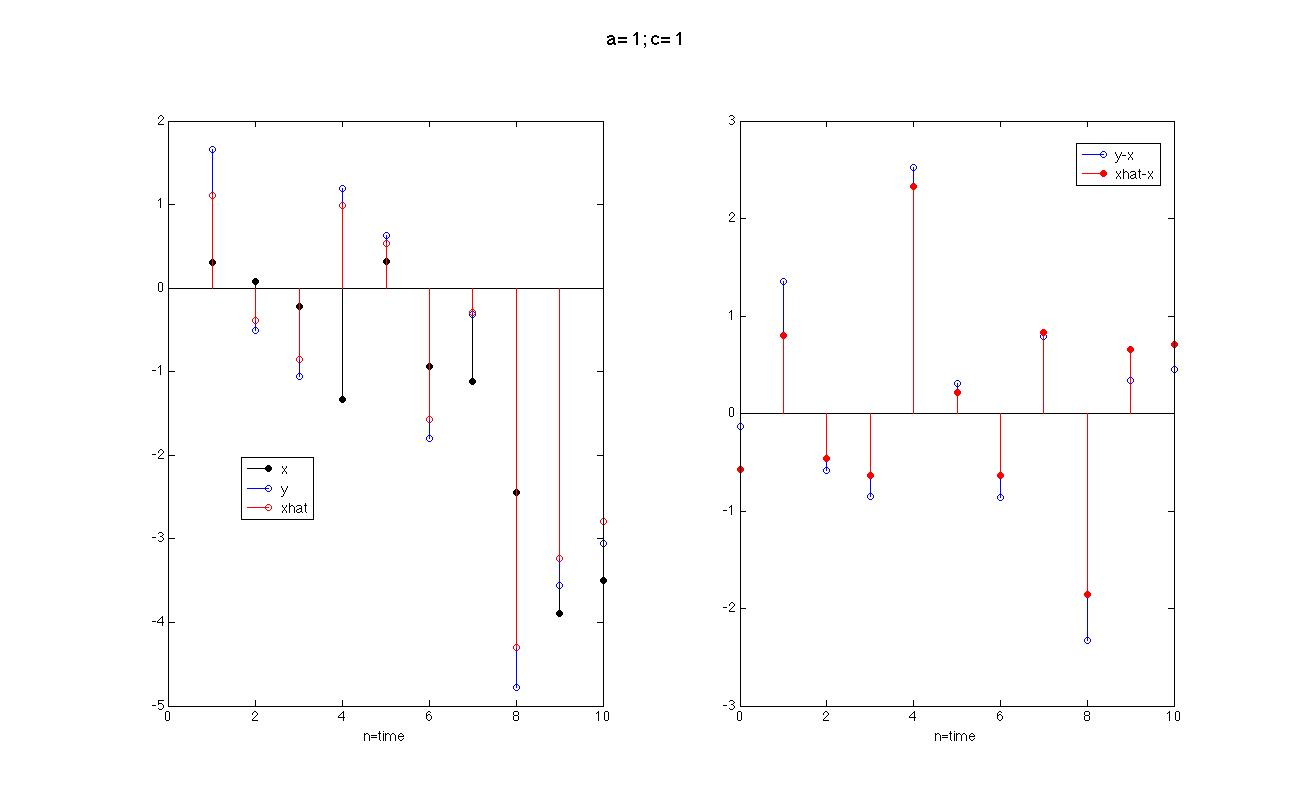
\includegraphics[scale=0.3]{fig4}\end{center}
In the beginning, our calculated xhat performs better in estimating x than the naive approach (y=x). Near the end, it appeared that y did better than xhat, but that was probably due to noise. A test over a longer period of time (n=100 instead of n=10) indicates that y converges toward xhat. This is because the noise in the observation approaches the expected value of 0.

\begin{center}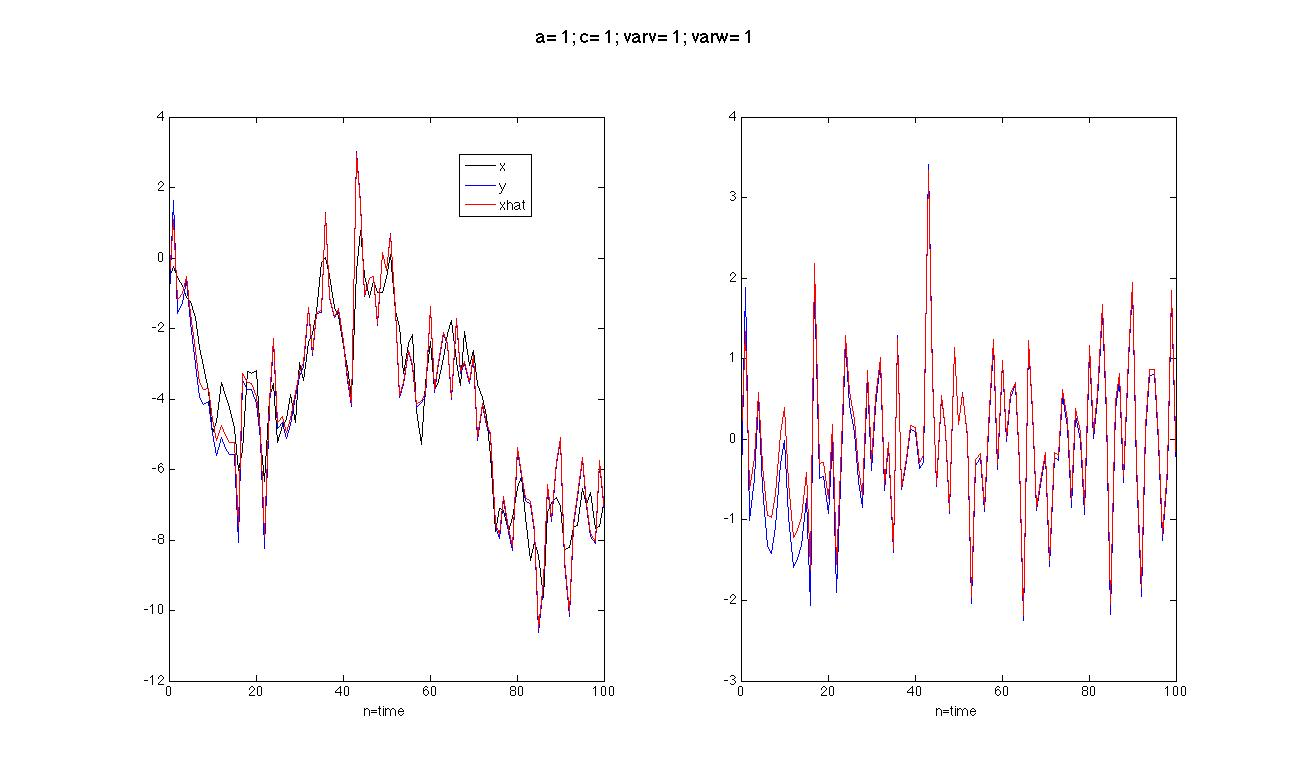
\includegraphics[scale=0.3]{fig11}\end{center}
\section{Varying A}
\begin{center}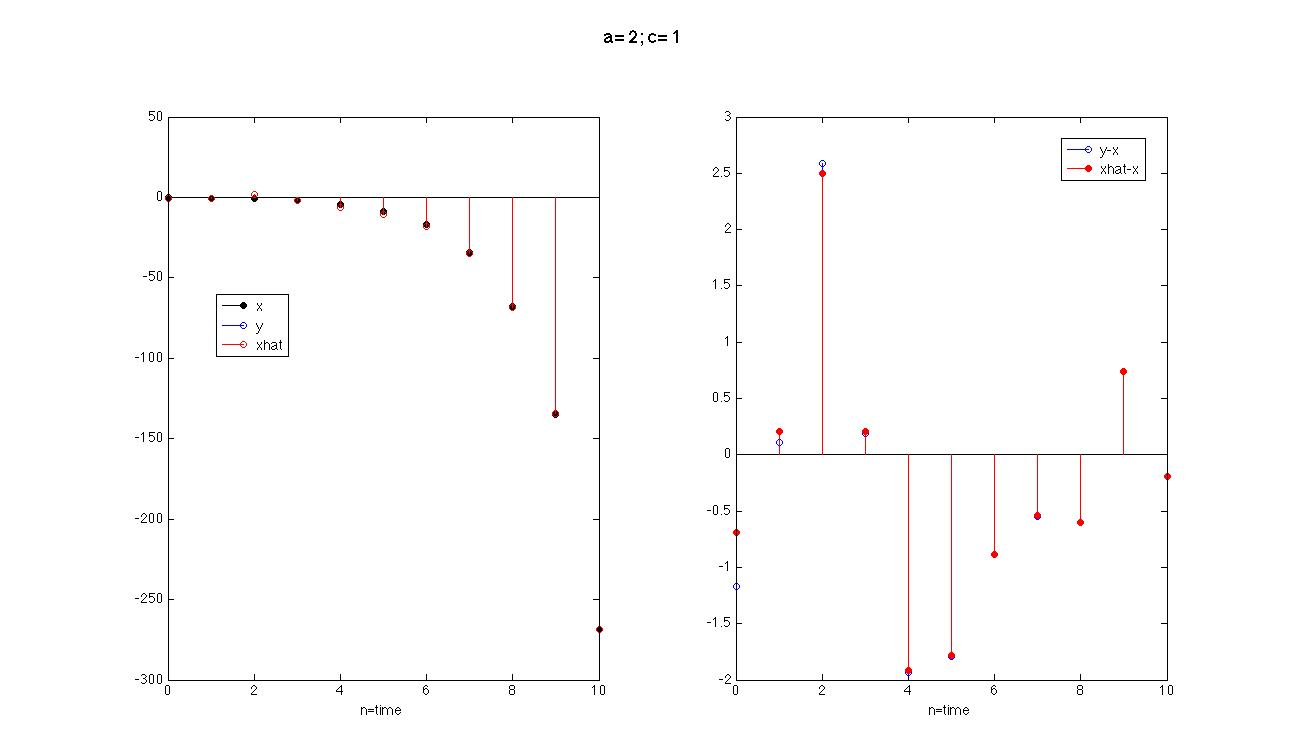
\includegraphics[scale=0.3]{fig1}\end{center}

When a is a fraction, there is greater resolution in the plot; since the y limits are smaller, we can see zoomed in the error of the observation and estimate. In addition, the noise has a greater effect on the system.

\begin{center}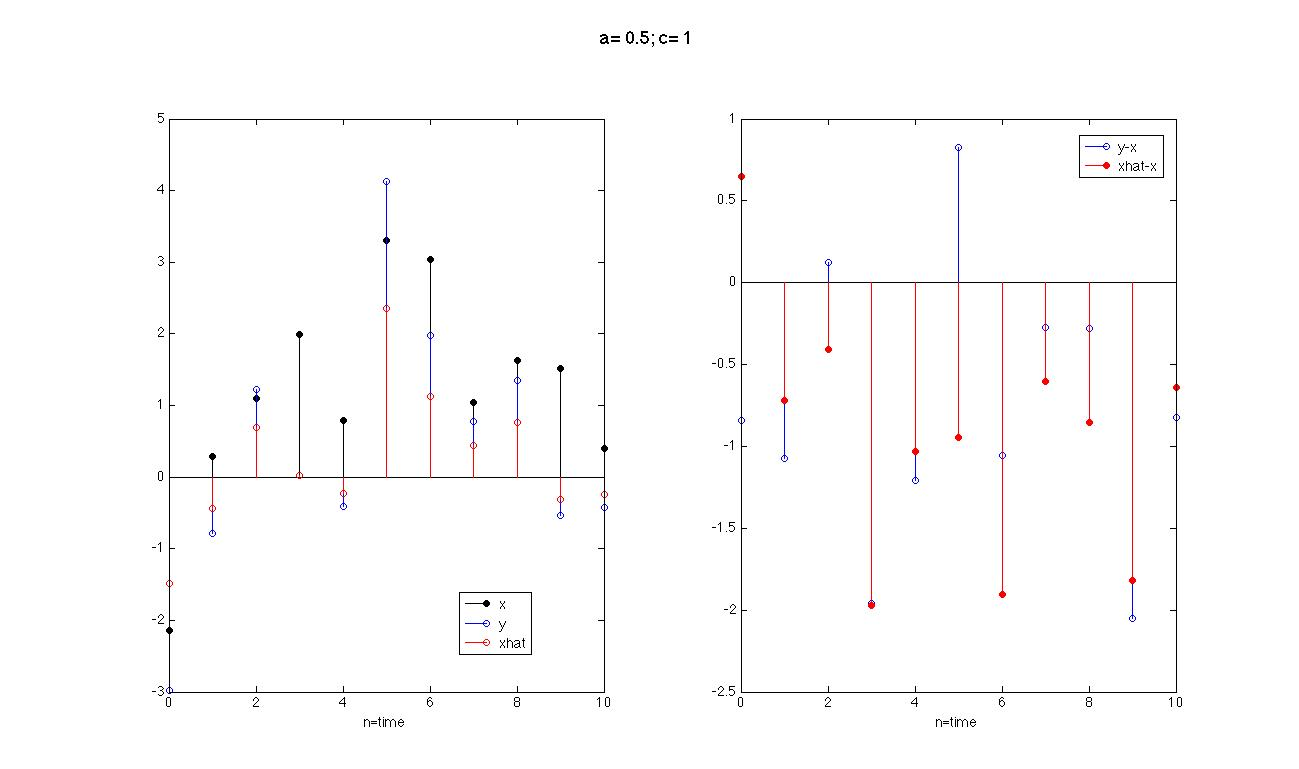
\includegraphics[scale=0.3]{fig2}\end{center}

\begin{center}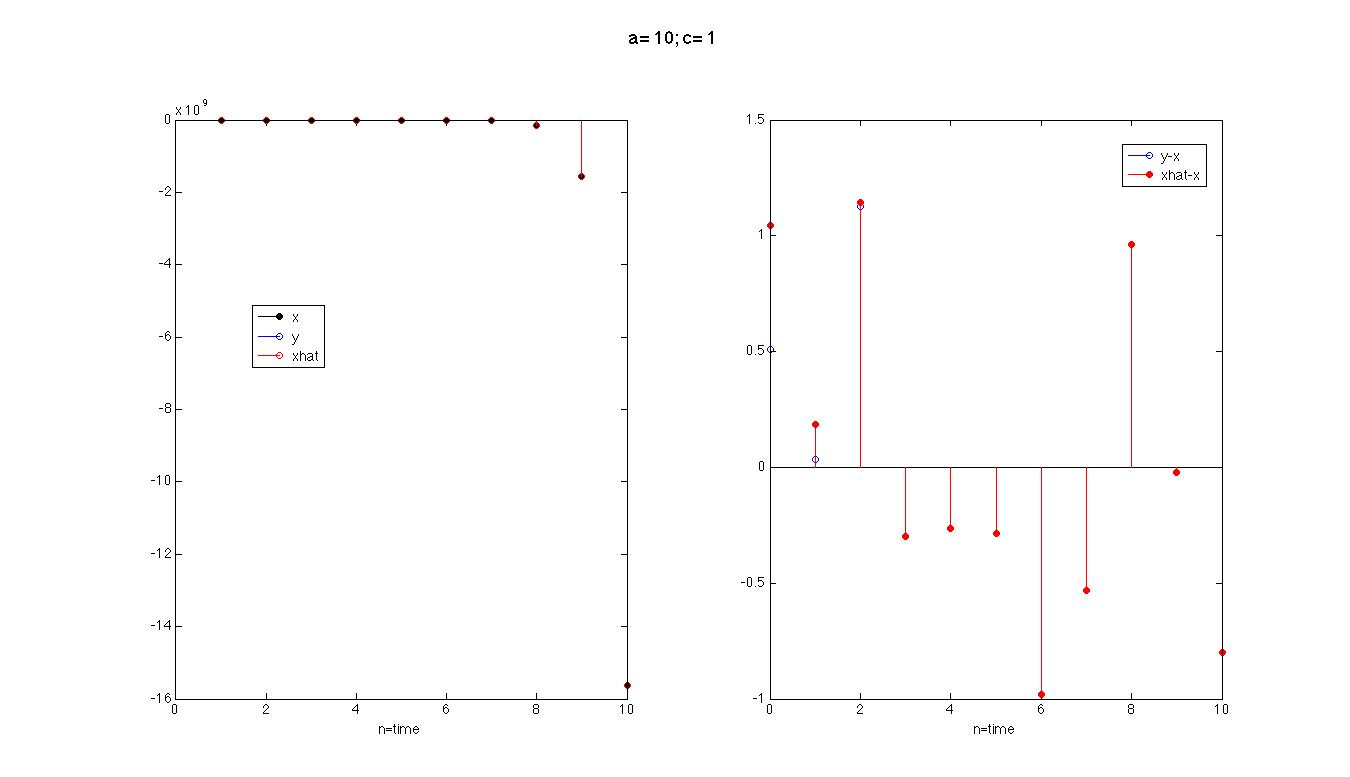
\includegraphics[scale=0.3]{fig3}\end{center}
Because a is so large, it's hard to see any difference between x and xhat. What is most important is that even though magnitude of x is in the order of $10^9$, the error remains $[-1.5,1.5]$. \textcolor{red}{Is there anything special about this interval?}

\section{Varying C}
\begin{center}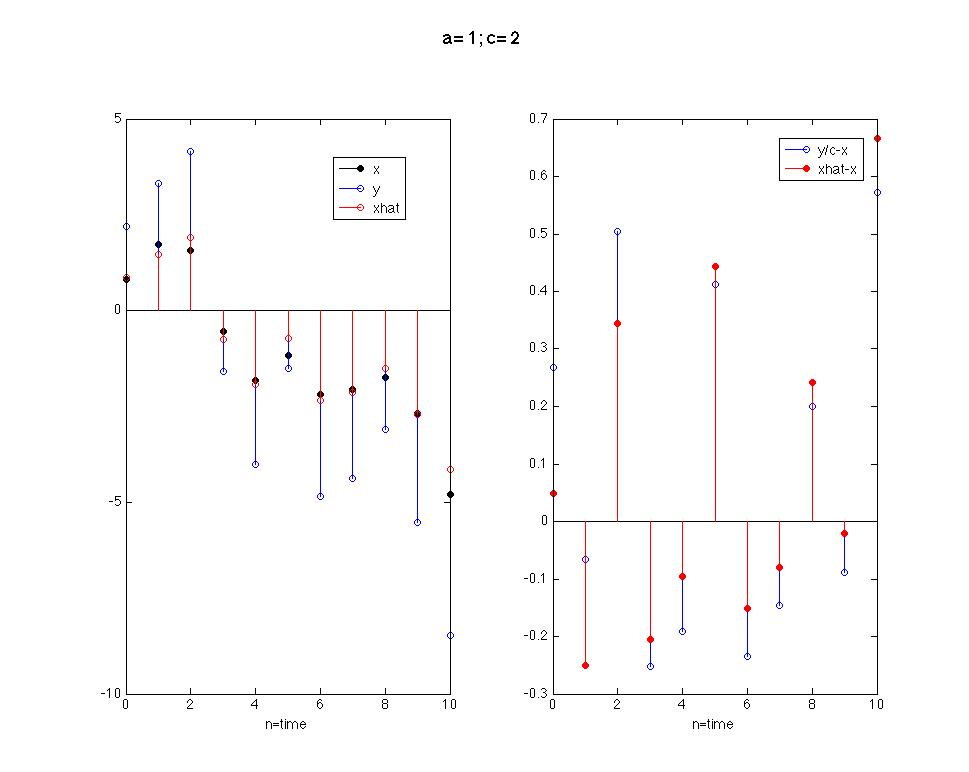
\includegraphics[scale=0.3]{fig5}\end{center}

\begin{center}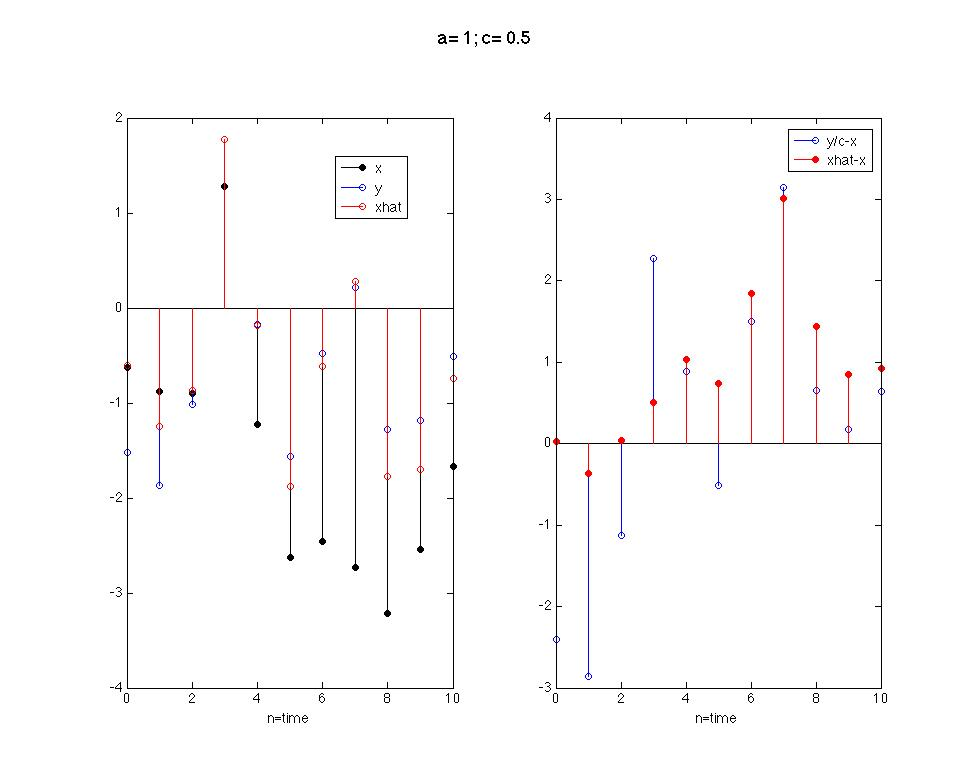
\includegraphics[scale=0.3]{fig6}\end{center}

\begin{center}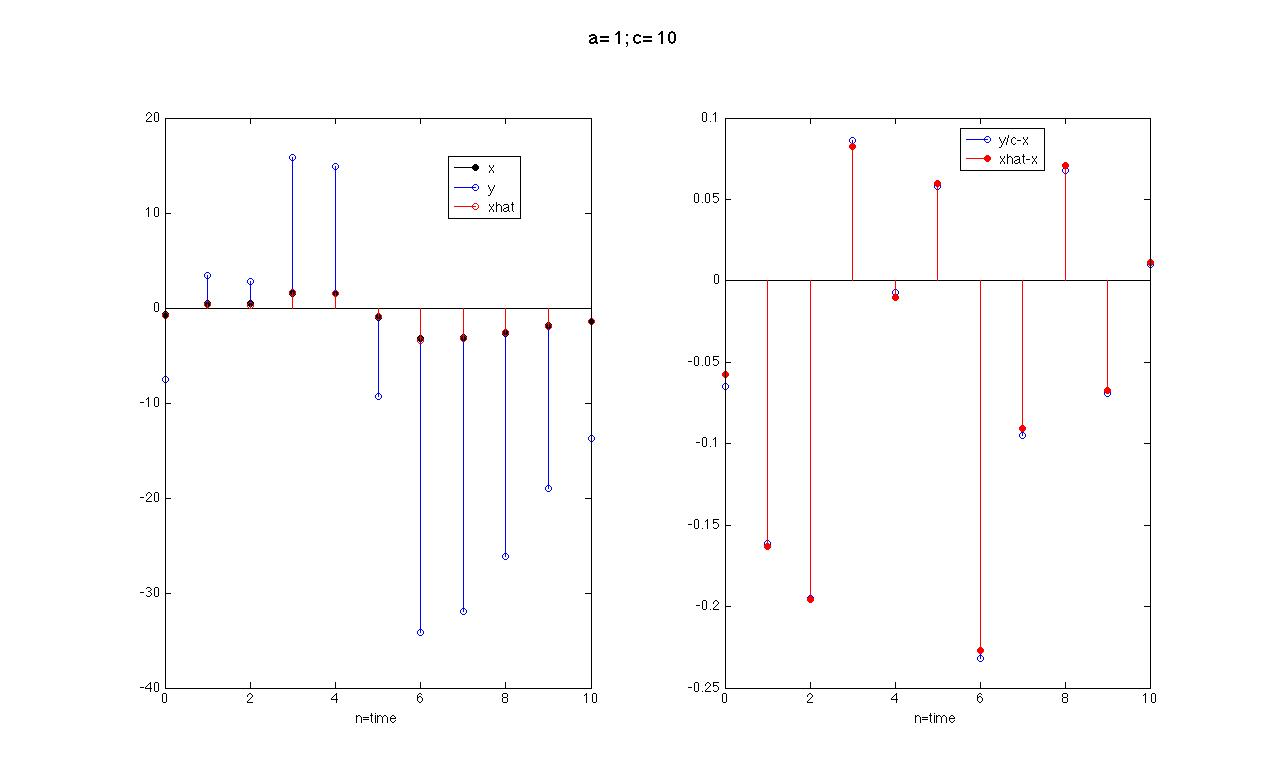
\includegraphics[scale=0.3]{fig7}\end{center}
When c increases the error in estimate decreases \textbf{significantly} (the same factor?). This might have something to do with the scaling decreasing the effect of noise in the system. It's interesting because c shouldn't affect the SNR at all.
\section{Varying Variance of Noise}
\begin{center}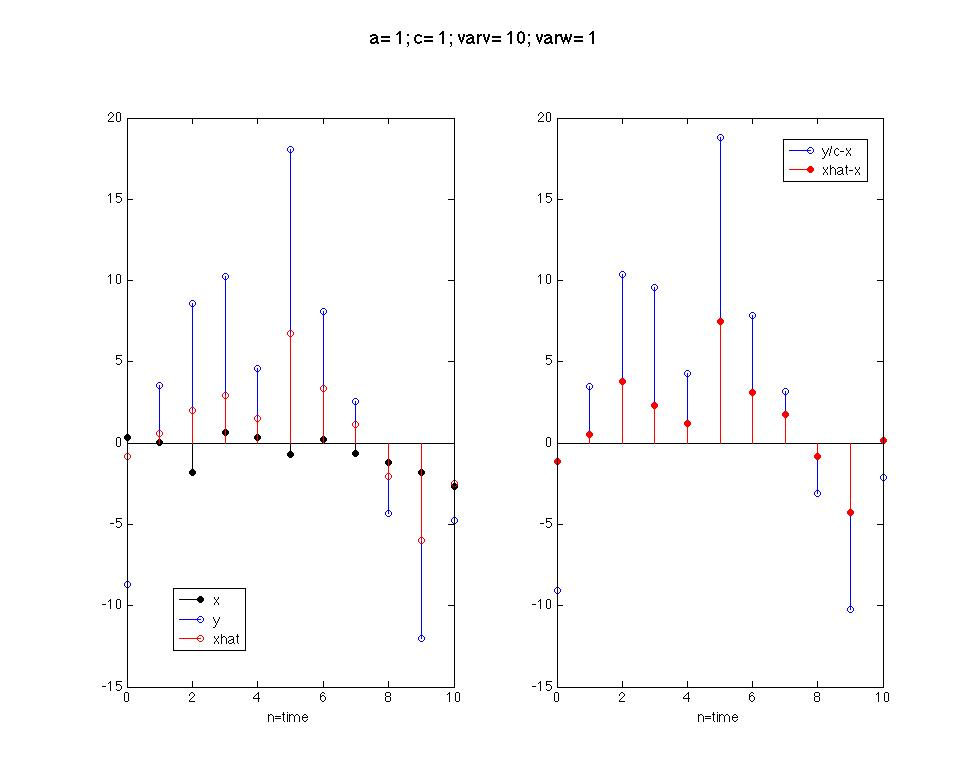
\includegraphics[scale=0.3]{fig8}\end{center}
Up until now, xhat and y/c were comparable in accuracy of estimating x. In this plot, I increased the noise of the observation so that it would affect y, and at every timestep xhat does better (thus proving xhat is a better estimator when noise can be significant.)

\begin{center}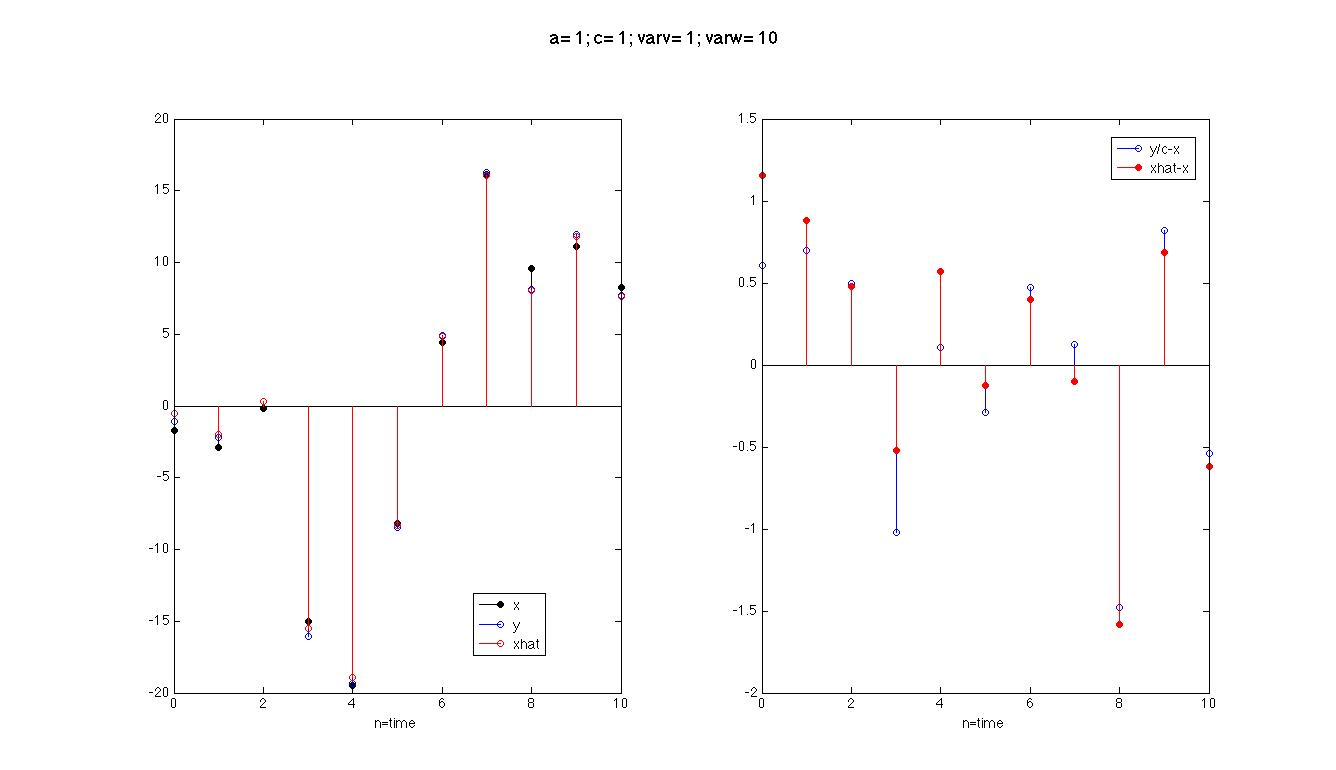
\includegraphics[scale=0.25]{fig9}\end{center}
In this plot, I increased the noise of the system. In this case, xhat and y are equally accurate at estimating x, with estimation error in the interval $[-1.5,1.5]$. There really is no benefit to using xhat instead of y/c.

\begin{center}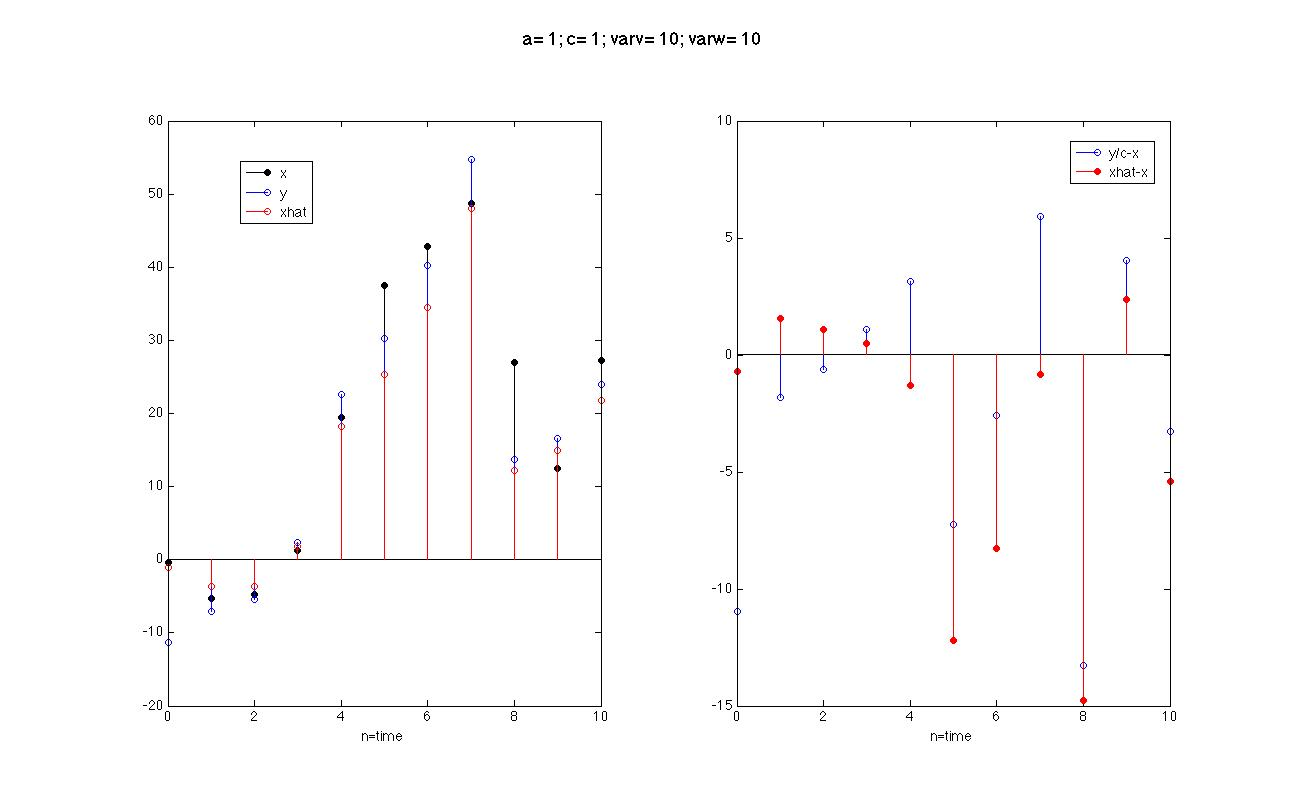
\includegraphics[scale=0.3]{fig10}\end{center}
In this plot, I increased the noise of both the system and the observation. Again, xhat isn't \textit{that} much better than y/c. This shows xhat is only useful when the noise of observation outweighs noise of the system.

\end{document}